\documentclass{report}

\input{~/dev/latex/template/preamble.tex}
\input{~/dev/latex/template/macros.tex}

\title{\Huge{Calculus 1 Notes}}
\author{\huge{Nathan Warner}}
\date{\huge{December 17, 2023}}
\graphicspath{{../images}}

\begin{document}
    \maketitle

    \begin{center}
        \Huge{Chapter 2}
    \end{center}
    \line(1,0){470} 

    \bigbreak \noindent \bigbreak \noindent  
    \begin{Huge}
        \noindent \textbf{Contents}
    \end{Huge}
    
    \bigbreak \noindent \bigbreak \noindent 
    \begin{Large}
        \textbf{2.1: The Tangent and Velocity Problems } 1-7
        \bigbreak \noindent \bigbreak \noindent  
        \textbf{2.2.1 The Limits of a Function } 8-12
        \bigbreak \noindent \bigbreak \noindent  
        \textbf{2.2.2 Infinite Limits }
        \bigbreak \noindent \bigbreak \noindent 
        \textbf{2.2.3 Finding Limits of a Trigonometric Function }
        \bigbreak \noindent \bigbreak \noindent 
        \textbf{2.3 Calculating Limits Using Limit Laws} 13-18
        \bigbreak \noindent \bigbreak \noindent 
        \textbf{2.5.1 Continuity } 19-30
        \bigbreak \noindent \bigbreak \noindent 
        \textbf{2.5.2 One-Sided Continuity}
        \bigbreak \noindent \bigbreak \noindent 
        \textbf{2.6 Limits at Infinity: Horizontal Asymptotes}
        \bigbreak \noindent \bigbreak \noindent  
        \textbf{2.7 Derivatives and Rates of Change}
        \bigbreak \noindent \bigbreak \noindent 
        \textbf{2.8.1 The Derivative of a Function}
        \bigbreak \noindent \bigbreak \noindent 
        \textbf{2.8.2 Finding The Derivatives Using The Limit Definition}
    \end{Large}

    \pagebreak
    \begin{Large}
        \noindent \textbf{2.1: The Tangent and Velocity Problems}
    \end{Large}

    \bigbreak \noindent \bigbreak \noindent \bigbreak \noindent 
    \begin{large}
       \noindent \textbf{The Tangent Problem: } 
    \end{large}
   
    \bigbreak \noindent 
    \qs{}{Can we find an equation of the tangent line to $y=x^2$ at the point P(1,1)?}
   
    \bigbreak \noindent 
    \begin{center}
        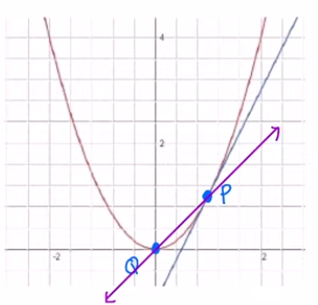
\includegraphics[scale=0.8]{14.png}    
    \end{center}
    
    \pf{Explanation}{. \\
        $y=x^2$: Red parabola \\
        Tangent line: Blue line \\ 
        Secent Line: Pink line with points q and p
    }

    We are asked to get the equation of the tangent line to $y=x^2$ at the point P(1,1), 
    However to find the equation of this line we know we need \textbf{2 things,} 
    \begin{itemize}
        \item Point
        \item Slope
    \end{itemize}

    \noindent Since we only have one point, we cannot find slope. Therefore, we must use 
    another point as an approximation and create a secent line instead. \textbf{This secent line is 
    the pink line in the above graphic.}
    
    \bigbreak \noindent 
    \textbf{So}, lets use the point Q(0,0) as our second point. Now we can find slope with 
    P(1,1), and Q(0,0).

    \bigbreak \noindent 
    \begin{large}
        \textbf{If} Slope = $\frac{y2-y1}{x2-x1}$, Then M of PQ $\rightarrow$ $ \frac{1-0}{1-0}$ = 1
    \end{large}

    \bigbreak \noindent 
    \textbf{Lets} get a better approximation by using a point closer to the tangent line
    Lets use Q(0.9, 0.81)

    \bigbreak \noindent 
    \begin{large}
        \textbf{So} M of PQ $\rightarrow$ $\frac{1-0.81}{1-0.9}$ = 1.9
    \end{large}

    \bigbreak \noindent 
    \textbf{Now}, lets get an even closer approximation by using the point Q(0.99, 0.9801)
    
    \bigbreak \noindent 
    \begin{large}
       \textbf{So}, M of  PQ $\rightarrow$ $ \frac{1-0.9801}{1-0.99}$ = 1.99
    \end{large}

    \pagebreak
    \noindent \textbf{Notice}, as the point Q gets closer to P, the slope of PQ is getting closer to 2
    
    \bigbreak \noindent 
    \textbf{We write}, 
    \begin{center}
        \begin{large}
            $\lim\limits_{Q \to P}${M of PQ} = m
        \end{large}
    \end{center}

    \bigbreak \noindent 
    Where \textbf{m} on the right of equation is slope of tangent line at \textbf{P}, 
    And \textbf{M of PQ} is slope of the secent line

    \bigbreak \noindent \bigbreak \noindent 
    \begin{large}
        \textbf{Now,}     
    \end{large}
    \bigbreak \noindent 
    We will use our approximation of $m \approx 2$ to write the equation of the tangent line,
    using the orginial point P(1,1).

    \begin{align*}
        y-1=2\left(x-1\right) \\
        y-1=2x-2 \\
        y=2x-1
    .\end{align*}
    
    
    \pagebreak
    \begin{large}
       \noindent \textbf{The Velocity Problem:} 
    \end{large}
    
    \bigbreak \noindent \bigbreak \noindent 
    \begin{itemize}
        \item Average Velocity: $\frac{distance\ traveled}{time\ elapsed}$, which is 
            represented by the slope of the secent line.
        \item Instantaneous Velocity = Velocity at a given instant of time, which is represented 
            by the slope of the tangent line
    \end{itemize}

    \bigbreak \noindent \bigbreak \noindent  
    \ex{}{If a rock is thrown upward on the planet Mars, with a Velocity of 10 m/s, It's
    height in meters t seconds later is  given by $y=10t-1.86t^2$}

    \bigbreak \noindent 
    \qs{}{Find the average Velocity over the given time intervals:}
    
    \bigbreak \noindent 
    \textbf{(i)} \textbf{[1,2]} $\rightarrow$ 1 and 2 represent values of \textit{t}
    
    \bigbreak \noindent 
    \begin{center}
        Substitute values into equation above
    \end{center}
    \begin{align*}
        y\left(1\right)=10\left(1\right)-1.86\left(1\right)^2 \\
        = 8.14
    .\end{align*}

    \begin{align*}
        y\left(2\right)=10 \left(2\right) - 1.86 \left(2\right) ^2 \\
        = 12.56
    .\end{align*}

    \bigbreak \noindent 
    \textbf{If} Average Velocity = $\frac{distance\ traveled}{time\ elapsed}$ Or better yet
    $ \frac{Change\ in\ height}{change\ in\ time}$

    \bigbreak \noindent 
    \textbf{And} we have the points (1,8.14) and (2,12.56)

    \bigbreak \noindent 
    \textbf{Then,}

    \begin{align*}
        Average\ Velocity = \frac{12.56-8.14}{2-1} \\
        =4.42 m\diagdown s
   .\end{align*}

    \pagebreak
    \textbf{(ii) [1,1.5]}
    
    \begin{center}
        Substitute values into equation above
    \end{center}
    \begin{align*}
        y\left(1\right)=10\left(1\right)-1.86\left(1\right)^2 \\
        = 8.14
    .\end{align*}

    \bigbreak \noindent 
    \begin{align*}
        y \left(1.5\right) = 10 \left(1.5\right) - 1.86 \left(1.5\right) ^2 \\
        =10.815 
    .\end{align*}

    \bigbreak \noindent 
    \textbf{After} solving theses equations we have the points (1,8.14) and (1.5,10.815)
    \bigbreak \noindent 
    \textbf{So,}
    
    \begin{align*}
        Average\ Velocity = \frac{10.815-8.14}{1.5-1} \\
        = 5.35 m \diagdown s
    .\end{align*}


    \pagebreak
    \begin{Large}
        \textbf{2.2.1 The Limit of a Function:}
    \end{Large}
    
   \bigbreak \noindent \bigbreak \noindent  
    \qs{}{Consider the values of $f \left(x\right) = x^2$ + 2 near $x=2$}

    \bigbreak \noindent 
    We want to know whats going on near x=2, so we make a table

    \bigbreak \noindent 
    \begin{center}
        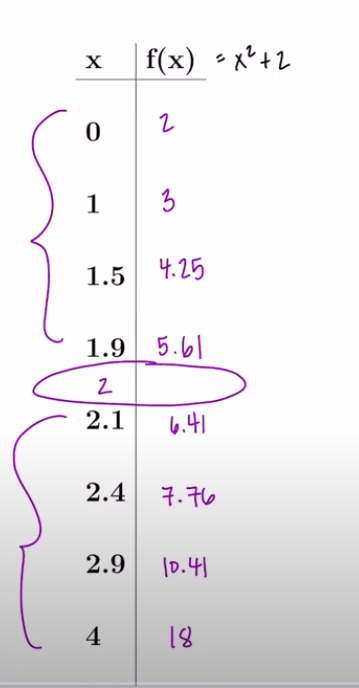
\includegraphics[scale=0.5]{../images/tbale.png}
    \end{center}

    \textbf{Now} we want to look at the closet x values to 2, 
    which is the 2 that are above and below \textbf{2}, \textbf{We observe that as x values approach
    2, then f(x) values approach 6}

    \bigbreak \noindent 
    \textbf{so we write,}    

    \begin{large}
        \begin{align*}
            \lim\limits_{x \to 2}{f \left(x\right) = 6}
        .\end{align*}
    \end{large}
    
    \bigbreak \noindent 
    \ex{}{Use a table of values to estimate the limit:$\lim\limits_{x \to 0 }{ \frac{tan3x}{tan5x}}$}
    
    \bigbreak \noindent 
    Rememeber the value \textbf{0} is \textbf{a} so we want to contruct our table where a 
    is in the middle, so use values that are smaller and larger than a.

    \bigbreak \noindent 
    Using arbitrary values that are close to 0, we get the table, 

    \bigbreak \noindent 
    \begin{center}
        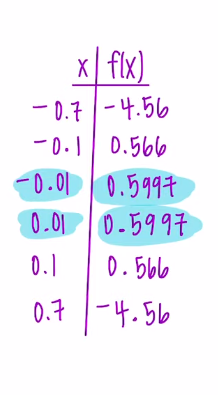
\includegraphics[scale=0.5]{../images/table2.png}
    \end{center}
    
    \bigbreak \noindent 
    Now after looking at our table, we can conclude that

    \bigbreak \noindent 

    \begin{large}
        \begin{align*}
            \lim\limits_{x \to0 }{ \frac{tan3x}{tan5x} = 0.6}
        .\end{align*}
    \end{large}

    \pagebreak
    \begin{large}
        \noindent \textbf{One Sided Limits:}
    \end{large}
   
    
    \bigbreak \noindent 
    \begin{center}
        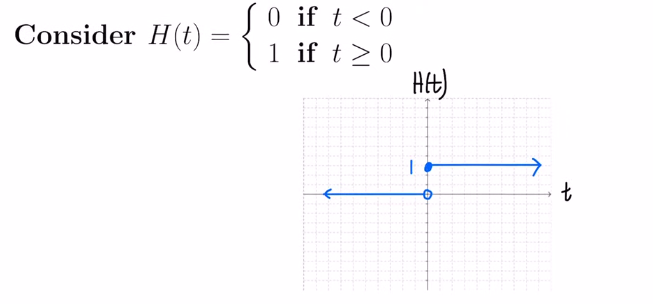
\includegraphics[scale=0.5]{../images/ht.png} 
    \end{center}

    \bigbreak \noindent \bigbreak \noindent 
    \nt{if there is a \textbf{minus} sign after a, that means you are approaching limit from the left
        if there is a \textbf{plus} sign after a, that means you are approaching limit from the right, 
        if you see a limit with either of these, it is called a two sided limit
    }
    \bigbreak \noindent 
    \textbf{What is $\lim\limits_{t \to 0- }{h \left(t\right)}$}

    \bigbreak \noindent 
    So looking at the bottom line, coming from the left, as we approach 0, the y value is 
    0.

    \bigbreak \noindent 
    \textbf{so $\rightarrow$}

    \begin{align*}
        \lim\limits_{t \to 0- }{h \left(t\right) = 0}
    .\end{align*}


    \bigbreak \noindent 
    \textbf{What is $\lim\limits_{t \to 0+}{h \left(t\right)}$} 

    \bigbreak \noindent 
    Given that we are approaching from the right, we are now looking at the top line, 
    we can see that as we approach 0, y is 1

    \bigbreak \noindent 
    \textbf{so}

    \begin{align*}
        \lim\limits_{t \to 0+ }{h \left(t\right) = 1}
    .\end{align*}

    \bigbreak \noindent 
    \nt{The first one is our \textbf{Left hand limit} and the bottom one is our \textbf{right hand limit} 
        if the side we our approaching from is not specified, \textbf{we cannot find the limit, so we would say DNE}
    }

    \bigbreak \noindent 
    \textbf{So}

    \bigbreak \noindent 
    $\lim\limits_{x \to 0}{f \left(x\right) = l}$ \textbf{iff} (if and only if) $\lim\limits_{x \to 0- }{f \left(x\right) = L}$ \textbf{and} $\lim\limits_{x \to 0+ }{f \left(x\right) = L}$

    \bigbreak \noindent 
    in other words, we can only drop the + or - after the a if the right and left hand limits are the same

    \pagebreak
    \begin{large}
       \noindent \textbf{Infinite Limits:} 
    \end{large}
    
    \bigbreak \noindent \bigbreak 
    \begin{center}
        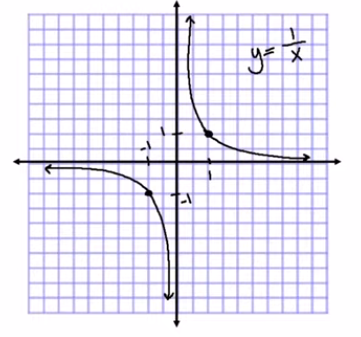
\includegraphics[scale=0.7]{../images/graph.png}
    \end{center}
    
    \bigbreak \noindent 
    \textbf{if we look at }

    \begin{large}
        \begin{align*}
            \lim\limits_{x \to 0+}{f(x) = ?}
        .\end{align*}
    \end{large}
    
    \bigbreak \noindent 
    We notice that as we approach 0 from the right, f(x) goes to infinity

    \bigbreak \noindent 
    \textbf{So:}
    
    \begin{large}
        \begin{align*}
            \lim\limits_{x \to 0+}{f(x) = \infty}
        .\end{align*}
    \end{large}
    
    \bigbreak \noindent 
    This is also the same for x $\rightarrow$ $0-$
    
    \bigbreak \noindent 
    \textbf{So:}

    \begin{large}
        \begin{align*}
            \lim\limits_{x \to 0-}{f \left(x\right) = -\infty}
        .\end{align*}
    \end{large}

    \bigbreak \noindent 
    \nt{x = 0 is a vertical Asymptote}

    \begin{center}
        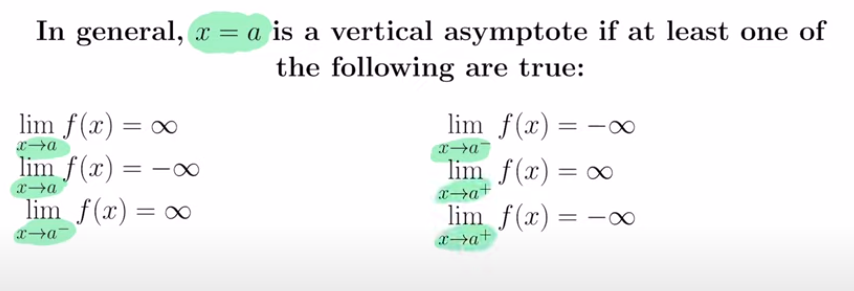
\includegraphics[scale=0.5]{../images/ass.png}
    \end{center}

    \bigbreak \noindent \bigbreak \noindent 
    \begin{large}
       \textbf{Examples: Determine the infitite limit} 
    \end{large}

    \bigbreak \noindent 
    \begin{large}
       \textbf{1.)} $\lim\limits_{x \to 5-}{ \frac{x+1}{x-5}}$ 
    \end{large}
    
    \bigbreak \noindent \bigbreak \noindent 
    \begin{center}
        \begin{large}
            x + 1 $\longrightarrow$ 6 \\
            x - 5 $\longrightarrow$ 0 
        \end{large}
    \end{center}

    \bigbreak 
    \begin{large}
        If you have a $ \frac{nonzero\ constant}{approaching\ 0} $ 
        its either going to be approaching $\infty$ or $-\infty$ the way we find which version of infinity
        it will be is with either a table or a numberline
    \end{large}
    
    \bigbreak 
    To make the numerline we want to list the zeros, so -1 and 5. Then pick a value thats close to a
    and approachs in the correct direction. Then plug this number into the equation and whatever sign you get
    will be the sign for infinity.
    \bigbreak \noindent 
    \begin{center}
        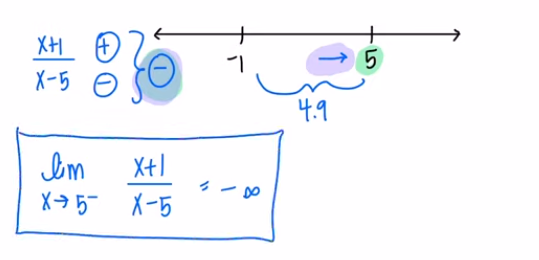
\includegraphics[scale=.5]{../images/line.png}
    \end{center}
    
    \bigbreak \noindent \bigbreak \noindent  
    \begin{large}
        \textbf{2.)} $\lim\limits_{x \to 5-}{ \frac{e^x}{ \left(x-5\right)^3}}$ 
    \end{large}

    \bigbreak \noindent 
    \begin{center}
       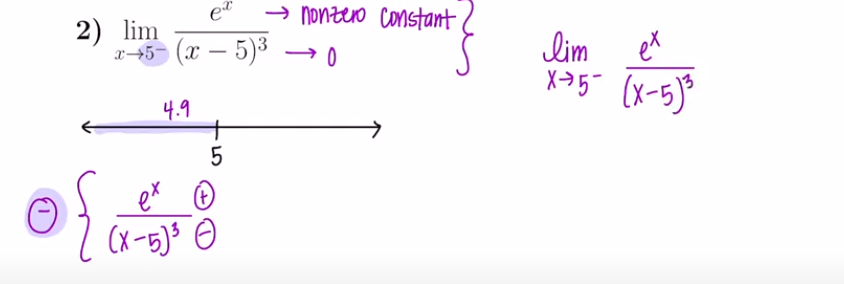
\includegraphics[scale=0.5]{ ../images/abc.png } 
    \end{center}
    
   \pagebreak
   \begin{Large}
      \noindent \textbf{2.3: Calculating using limit laws} 
    \end{Large}
  
    \bigbreak \noindent \bigbreak \noindent 
    \begin{large}
        \begin{center}
            \textbf{The limit laws:} 
        \end{center}
    \end{large}
   
    \bigbreak \noindent 
    \begin{center}
        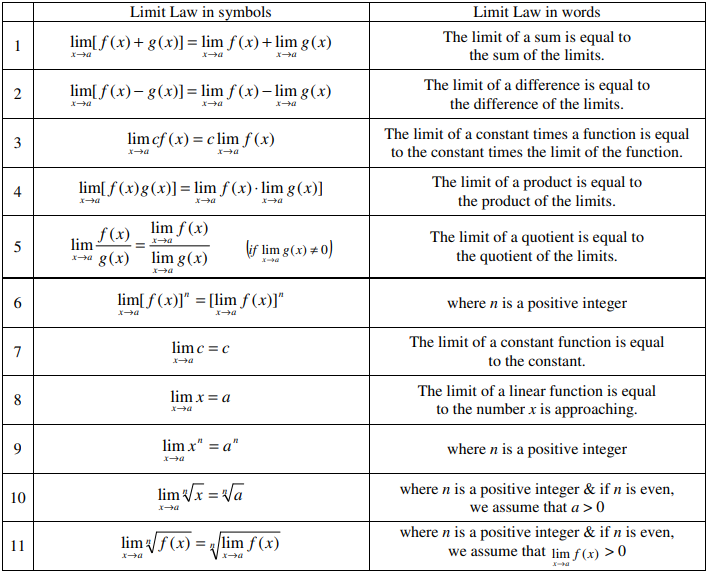
\includegraphics[scale=0.65]{ ../images/laws.png }
    \end{center}
    
    \bigbreak \noindent \bigbreak \noindent 
    \qs{}{Find the limit if $\lim\limits_{x \to 2}{f \left(x\right) = 4}$ and $\lim\limits_{x \to -2}{f \left(x\right) = -2}$}
    \bigbreak \noindent 
    \textbf{ $\lim\limits_{x \to 2}{f \left(x\right)+5g \left(x\right)}$}
    
    \bigbreak \noindent 
    \pf{Solution}{}
    \noindent Using limit laws 1 and 3 we can solve this problem

    \begin{align*}
    \lim\limits_{x \to 2}{f \left(x\right)} + \lim\limits_{x \to 2}{5g \left(x\right)} \rightarrow \textbf{law\ 1} \\ 
        \lim\limits_{x \to 2}{f \left(x\right)} + 5 \lim\limits_{x \to 2}{g \left(x\right)} \rightarrow \textbf{Law\ 3} \\ 
        4 + 5 \left(-2\right) = -6
    .\end{align*}

   \pagebreak
    \qs{}{Given $\lim\limits_{x \to 2}{g \left(x\right)= -2}$ $\lim\limits_{x \to 2}{h \left(x\right) = 0}$
        find $\lim\limits_{x \to 2}{ \frac{g \left(x\right)}{h \left(x\right)}}$
    }

    \bigbreak \noindent 
    \pf{Solution}{}
    Using limit law 5 we can solve this

    \begin{align*}
        \frac{ \lim\limits_{x \to 2}{g \left(x\right)}}{ \lim\limits_{x \to 2}{h \left(h\right)}} = \frac{-2}{0} \\
        \textbf{DNE}
    .\end{align*}

    \bigbreak \noindent 
    \begin{large}
       \textbf{Direct Substitution Property:} 
    \end{large}

    \bigbreak \noindent 
    \dfn{}{if f is a polynomial or a rational function and a is in the domain of f, then 
        $\lim\limits_{x \to a}{f \left(x\right)= f \left(a\right)}$
    }

    \bigbreak \noindent 
    \begin{large}
       \textbf{Example:} 
       $\lim\limits_{x \to 2}{ \frac{2x^2+1}{x^2+6x-4}}$
    \end{large}

    \bigbreak \noindent \bigbreak \noindent 
    \textbf{a) what function is this?}
    \pf{Answer}{} 
    \noindent This is a \textbf{rational} function 


    \bigbreak \noindent \bigbreak \noindent  
    \textbf{b) is 2 in the domain of the function?}
    \pf{Answer}{}
    \noindent if we plug in 2 in the denomonator, the function does not equal 2, 
    so \textbf{Yes}, 2 is in the domain of this function, therefore, we can solve for f(a)
    and get the limit of this function

    \begin{align*}
        \frac{2 \cdot 2^2+1}{2^2+6*2-4} \\
        = \frac{9}{12} \\
        = \frac{3}{4}
    .\end{align*}

    \bigbreak \noindent 
    \begin{large}
       \textbf{Example 3: Evaluate the limit, if exists:} 
        \bigbreak \noindent 
        $\lim\limits_{x \to 1}{ \frac{x^3-1}{x^2-1}}$
    \end{large}
    
   \pf{Solution}{} 
   \noindent In this case, if we plug in 1 to the denomonator, we get 0. Therefore \textbf{a} is not in the domain of \textbf{f}. 
   So we must attempt to find the limit of this function with \textbf{Factoring}

   \pagebreak
   \begin{large}
      \noindent \textbf{Review: Factoring sums or difference of cubes:} 
   \end{large}

   \bigbreak \noindent \bigbreak \noindent 
   Difference of cubes: $a^3-b^3 = \left(a-b\right) \left(a^2+ab+b^2\right)$ 
   \bigbreak \noindent 
   Sum of cubes: $a^3+b^3 = \left(a+b\right) \left(a^2-ab-b^2\right)$

   \bigbreak \noindent \bigbreak \noindent 
   \begin{large}
      \noindent \textbf{Example of difference of cubes} 
   \end{large}
    
   \bigbreak \noindent 
   \textbf{a) $x^3-8$}

    \bigbreak \noindent 
    This is \textbf{$a^3-b^3$}, Where a = x and b = 2 because $2^3 = 8$

    \bigbreak \noindent 
    \textbf{So:}
 
    \begin{align*}
        \left(x-2\right) \left(x^2+2x+4\right)
    .\end{align*}
    
    \bigbreak \noindent 
    \textbf{Back to Example 3:}
    So using difference of cubes we get
    
    \begin{align*}
        \lim\limits_{x \to 1}{\frac{ \left(x-1\right) \left(x^2+x+1\right)}{ \left(x-1\right) \left(x+1\right)}} 
    .\end{align*}
    
    \bigbreak \noindent 
    \noindent Now if we \textbf{cancel} out \textbf{common factors, we get: }

    \begin{align*}
        \lim\limits_{x \to 1}{ \frac{ \left(x^2+x+1\right)}{ \left(x+1\right)}}
    .\end{align*}

    \bigbreak \noindent 
    Now with this new equation, \textbf{1 is} in the domain. So we plug 1 into the new equation and get:

    \begin{align*}
        \frac{1^1+1+1}{1+1} \\
        = \frac{3}{2}
    .\end{align*}

    \bigbreak \noindent \bigbreak \noindent  
    \begin{large}
        \textbf{Example 4: $\lim\limits_{h \to 0}{ \frac{\sqrt{9+h} -3}{h}}$ } 
    \end{large}

    \bigbreak \noindent \bigbreak \noindent  
    Straight away, we can see that h = 0 is \textbf{not} in the domain of the function. 
    So we want to try and get rid of this radical in the numerator by multiplying by the
    conjugate
    
    \bigbreak \noindent 
    \textbf{So:}

    \begin{align*}
        \lim\limits_{h \to 0}{ \frac{\sqrt{9+h} - 3}{h}} \cdot \frac{ \left(\sqrt{9+h} +3\right)}{ \left(\sqrt{9+h} +3\right)} \\       
        = \lim\limits_{h \to 0}{ \frac{9+h-9}{h \left(\sqrt{9+h}+3\right)}} \\ 
        = \lim\limits_{h \to 0}{ \frac{h}{h \left(\sqrt{9+h}+3\right)}} \\
        = \lim\limits_{h \to 0}{ \frac{1}{\sqrt{9+h}+3}} \\
    .\end{align*}

    \noindent \textbf{Now with this new equation, 0 is in the domain, so we can plug in 0.}

    \begin{align*}
        = \frac{1}{\sqrt{9+0}+3} \\
        = \frac{1}{6}
    .\end{align*}

    \bigbreak \noindent \bigbreak \noindent 
    \begin{large}
       \textbf{Example 5: $\lim\limits_{x \to 4}{ \frac{x^2-4x}{x^2-3x-4}}$} 
    \end{large}
   
    \bigbreak \noindent 
    Straight away we can see that if we plug 4 into the denomonator, we get 0. For this reason
    we know that 4 is not in the domain. Therefore we must factor
    
    \bigbreak \noindent 
    \textbf{So:}
    \begin{align*}
       \lim\limits_{x \to 4}{ \frac{x \left(x-4\right)}{ \left(x+1\right) \left(x-4\right)}} 
    .\end{align*}

    \bigbreak \noindent 
    After canceling out the common factor of $x-4$, we get the equation:

    \begin{align*}
        \lim\limits_{x \to 4}{ \frac{x}{x+1}}
    .\end{align*}

    \bigbreak \noindent 
    Now we can plug 4 into this new equation and get:

    \begin{align*}
        \frac{4}{5}
    .\end{align*}

    \bigbreak \noindent \bigbreak \noindent 
   \begin{large}
      \textbf{Example 6: $\lim\limits_{x \to -1}{ \frac{x^2-4x}{x^2-3x-4}}$} 
   \end{large}

   \bigbreak \noindent 
   Again we can see that -1 is not in the domain. However, with this example, if we factor
   out the equation and then plug -1 into our new equation, we get:

   \begin{align*}
       \frac{-1}{0}
   .\end{align*}
    
   \bigbreak \noindent 
   so we can see that the direct Substitution will not work. Therefore, our limit is either 
   $\infty$, or DNE, Rememeber that this is the case for $\frac{nonzero\ constant}{0}$. 
   Now we must test the equation to get the sign of $\infty$

   \bigbreak \noindent 
   \textbf{First test: Left side (Testing with -1.1)}

   \begin{align*}
       \lim\limits_{x \to -1-}{ \frac{x}{x+1}}
   .\end{align*}

   \bigbreak \noindent 
   If we plug -1.1 into the equation, we can see that both the numerator and the denomonator are negative, 
   therefore our sign is \textbf{Positive} $\infty$

   \bigbreak \noindent 
   \textbf{Second Test: Right side (testing with -0.9)}
   
   \bigbreak \noindent 
   If we plug -0.9 into the equation, we can see that the numerator is negative, but the denomonator
   is positive. Therefore our sign is \textbf{Negative} $\infty$

   \bigbreak \noindent 
   Because the \textbf{Left and Right hand limits are not the same}, we can deduce that the limit is DNE

   \bigbreak \noindent 
   \textbf{So:}

   \begin{align*}
       \lim\limits_{x \to -1}{ \frac{x^2-4x}{x^2-3x-4}} \\
       = DNE
   .\end{align*}
   
   \bigbreak \noindent \bigbreak \noindent 
   \begin{large}
       \noindent \textbf{Example 7: $\lim\limits_{x \to -6}{ \frac{2x+12}{\abs{x+6}}}$} 
   \end{large}

   \bigbreak \noindent \textbf{} 
   \nt{\textbf{Because we see absolute value in the denomonator, we want to rewrite as piecewise.}}
   
   \bigbreak \noindent \bigbreak \noindent 
   \begin{large}
      \textbf{Review of Piecewise:} 
   \end{large}

   \bigbreak \noindent \bigbreak \noindent 
   \textbf{Recall: }
  
   \bigbreak \noindent 
   \begin{equation}
    f(x)= \abs{x} =
        \begin{cases}
            x & \text{if } x \geq 0 \\ 
            -x & \text{if } x < 0 
        \end{cases}
    \end{equation}

    \bigbreak \noindent 
    \begin{large}
       \textbf{Example: abs as piecewise:} 
    \end{large}

    \begin{align*}
        g \left(x\right) = \abs{5-2x}
    .\end{align*}

    \bigbreak \noindent 
    First we want to figure out where the quantity inside the absolute value changes signs,
    to do this we set the quanity inside the absolute value \textbf{equal to 0}.
    
    \bigbreak \noindent 
    \textbf{So:}

    \begin{align*}
        5-2x=0 \\
        x= \frac{5}{2} 
    .\end{align*}

    \bigbreak \noindent 
    To visualize this, refer to this graph:

    \bigbreak \noindent 
    \begin{center}
        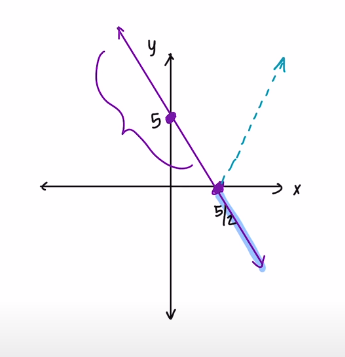
\includegraphics[scale=0.5]{../images/gr.png  }
    \end{center}

    \bigbreak \noindent \bigbreak \noindent
    We can see that the output values beyond $\frac{5}{2}$ will be reflected about the x-axis
    
    \bigbreak \noindent 
    So to write this Algebraically, Whever the zero is for the quanity inside the absolute value, 
    thats where we split the domain.

    \bigbreak \noindent 
    \textbf{So:}

    \bigbreak \noindent 
       \begin{equation}
        g(x)=
            \begin{cases}
                5-2x  & \text{if } x < \displaystyle{\frac{5}{2}} \\ 
                - \left(5-2x\right)      & \text{if } \displaystyle{ x \geq \frac{5}{2}} 
            \end{cases}
        \end{equation}

        \bigbreak \noindent 
        \begin{large}
           \textbf{Back to example 7:} 
        \end{large}
        
        \bigbreak \noindent 
        We want to rewrite the denomonator as a piecewise function.

        \bigbreak \noindent 
        \textbf{So:}

        \bigbreak \noindent 
           \begin{equation}
           \abs{x+6}=
                \begin{cases}
                    x+6 & \text{if } x \geq -6 \\ 
                    - \left(x+6\right) & \text{if } x < -6 
                \end{cases}
            \end{equation}

        \bigbreak \noindent 
        Now we want to rewrite the entire equation

        \bigbreak \noindent 
        \textbf{So:}

           \begin{equation}
               \frac{2 \left(x+6\right)}{\abs{x+6}}=
                \begin{cases}
                    \frac{2 \left(x+6\right)}{x+6} & \text{if } x > -6 \\ 
                    \frac{2 \left(x+6\right)}{-x+6} & \text{if } x < -6 
                \end{cases}
            \end{equation}

        \bigbreak \noindent 
        Now we can simplify this further by canceling out common factors x+6, and we are left with:

        \bigbreak \noindent 
           \begin{equation}
            \frac{2 \left(x+6\right)}{\abs{x+6}} =
                \begin{cases}
                     2 & \text{if } x > -6 \\
                     -2 & \text{if } x < -6 
                \end{cases}
            \end{equation}

        \bigbreak \noindent 
        Now we can find the limit, Since the direction is not specified, we must check at both sides.

        \bigbreak \noindent 
        \begin{align*}
            \lim\limits_{x \to -6- }{\frac{2x+12}{\abs{x+6}}} = -2
        .\end{align*}

        \bigbreak \noindent 
        The limit is -2 because if we approaching -6 from the left, we are looking
        at values that are smaller than -6, and if we look at our piecewise function, we can
        see that it would be -2 for values smaller than -6

        \begin{align*}
            \lim\limits_{x \to -6+}{\frac{2x+12}{\abs{x+6}}} = 2
        .\end{align*}        

        \bigbreak \noindent 
        Since left and right limits are not equal, this means that:

        \begin{align*}
            \lim\limits_{x \to -6}{\frac{2x+12}{\abs{x+6}}} \\ 
            = DNE
        .\end{align*}
        
        \pagebreak
        \begin{Large}
            \noindent \textbf{2.5: Continuity and the Intermediate Value Theorem:}
        \end{Large}

        \bigbreak \noindent \bigbreak \noindent \bigbreak \noindent 
        \begin{large}
            \textbf{Continuity:}
        \end{large}

        \bigbreak \noindent 
        \begin{center}
            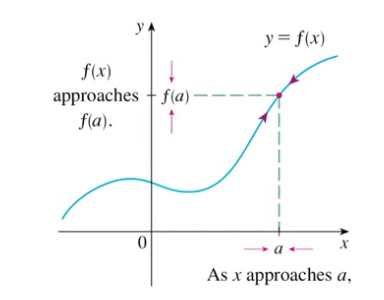
\includegraphics[scale=0.8]{../images/observe.png }
        \end{center}

        \bigbreak \noindent 
        What can we observe about f(x) at a?
        
        \bigbreak \noindent 
        \begin{itemize}
            \item f(x) is defined at a
            \item $\lim\limits_{x \to a}{f \left(x\right)}$ exists 
            \item $\lim\limits_{x \to a}{f \left(x\right) = f \left(a\right)}$
        \end{itemize}

        \bigbreak \noindent \bigbreak \noindent 
        \dfn{}{A function f is continuous at a if $\lim\limits_{x \to a}{f \left(x\right) = f \left(a\right)}$}

        \bigbreak \noindent
        \nt{Above 3 cases are required for f to be continuous at a, if that last bullet is true, then we know
            automatically that the first 2 bullets are also \textbf{\textit{satisfied}} 
        }

        \pagebreak
        \noindent \textbf{Example: Show f is continuous at a}

        \begin{align*}
            f \left(x\right) = x^2 + \sqrt{7-x}, a = 4 
        .\end{align*}

        \bigbreak \noindent
        Remember that a is the x value we are investigating. Show we need to show that 
        the 3 bullets above are true for this equation. 

        \bigbreak \noindent 
        \textbf{First} we need to find the domain of this function and see if \textbf{4} lies within
        that domain.

        \bigbreak \noindent 
        Since this function is a polynomial function \textbf{\textit{and a radical function}}, 
        we know that the domain of a polynomial function is $\mathbb{R}$. But because it is 
        also a radical function, we know we must set whats inside the radical $\geq$ 0 

        \bigbreak \noindent 
        \textbf{So if we solve the inequality:} 

        \begin{align*}
            x \leq 7
        .\end{align*}

        \bigbreak \noindent 
        \textbf{Therefore the domain of this function is:}

        \begin{align*}
            (-\infty, 7] 
        .\end{align*} 

        \bigbreak \noindent 
        \nt{Remember, when you solve for an inequality, and divide by a negative, 
            you must \textbf{\textit{flip the inequality}.}
        }

        \bigbreak \noindent 
        \textbf{Since 4 $\in$ D, then f(x) is defined at a=4}

        \bigbreak \noindent 
        \line(1,0){470}
        \bigbreak \noindent \bigbreak \noindent  
        \textbf{Second}, we need to show that $\lim\limits_{x \to 4}{f \left(x\right)}$ exists. 
        So we will first try to use direct Substitution and plug 4 into x:

        \begin{align*}
            \lim\limits_{x \to 4}{ \left(4\right)^2 + \sqrt{7-4}} \\ 
            = 16 + \sqrt{3}
        .\end{align*}

        \bigbreak \noindent \bigbreak \noindent 
        \textbf{Third}, we want to show that:
        
        \begin{align*}
            f \left(4\right) = \lim\limits_{x  \to 4}{x^2 + \sqrt{7-4}}
        .\end{align*}

        \bigbreak \noindent 
        So again, like step 2, we will plug in 4 for x:

        \begin{align*}
            f \left(4\right) = 4^2 + \sqrt{7-4} \\ 
            = 16 + \sqrt{3}
        .\end{align*}

        \bigbreak \noindent 
        \textbf{Since all 3 of these steps pass, we have shown Continuity at $ x = 4 $.}

        \pagebreak
        \begin{large}
            \noindent \textbf{Discontinuities:}
        \end{large} 

        \bigbreak \noindent \bigbreak \noindent 
        If we look at the following graph:

        \bigbreak \noindent 
        \begin{center}
            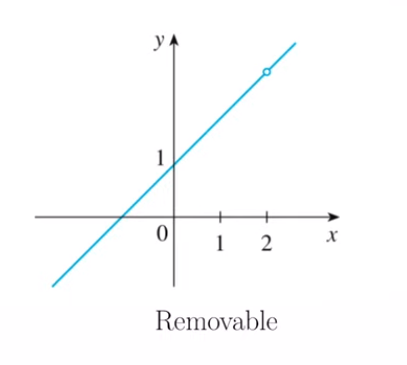
\includegraphics[scale=0.7]{../images/1.png}
        \end{center}

        \bigbreak \noindent 
        at we investigate a = 2, we can see that the $\lim\limits_{x \to 2}{f \left(x\right)}$
        does exist, \textbf{however,} f(x) is not defined at 2.

        \bigbreak \noindent \bigbreak \noindent 
        If we look at the following graph:

        \bigbreak \noindent 
        \begin{center}
            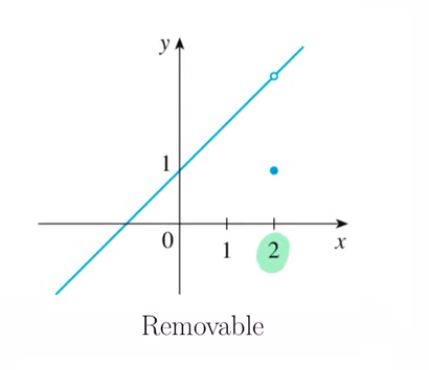
\includegraphics[scale=0.7]{../images/2.png}
        \end{center}

        \bigbreak \noindent 
        we can see that the $\lim\limits_{x \to 2}{f \left(x\right)}$ does exist, and 
        f(2) \textbf{\textit{is defined}}, However, $\lim\limits_{x \to 2}{f \left(x\right)}$ $\neq$ f(2)

        \bigbreak \noindent \bigbreak \noindent 
        \textbf{These 2 are \textit{Removable Discontinuities}} because the limit \textbf{does exist} at that point a = 2

        \bigbreak \noindent \bigbreak \noindent 
        Now if we look at: at a = 0 

        \bigbreak \noindent 
        \begin{center}
            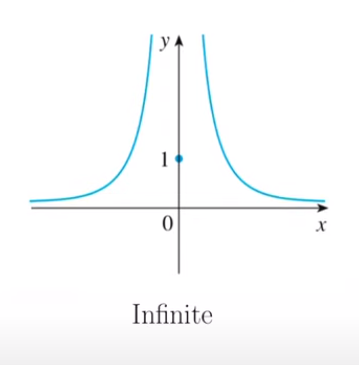
\includegraphics[scale=0.6]{../images/3.png}
        \end{center}

        \bigbreak \noindent 
        We can see that $\lim\limits_{x \to 0}{f \left(x\right) = \infty}$, Since the limit 
        is not a \textbf{\textit{finite number}}, that means that it is impossible for the 
        limit to equal the function value.

        \bigbreak \noindent \bigbreak \noindent 
        Now if we look at:

        \bigbreak \noindent 
        \begin{center}
            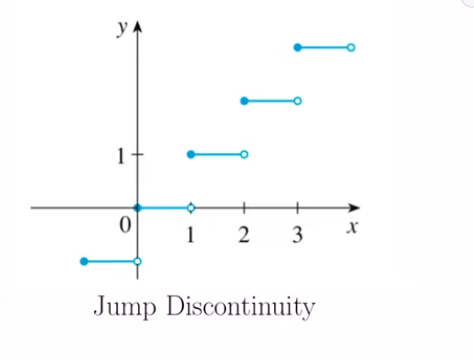
\includegraphics[scale=0.6]{../images/4.png}
        \end{center}

        \bigbreak \noindent
        We can see that the $\lim\limits_{x \to a}{f \left(x\right) = DNE, \text{where a is any integer}}$

        \pagebreak
        \noindent \textbf{Example: Explain why f is Discontinuous at a = 1, sketch the graph of f.}

        \bigbreak \noindent \bigbreak \noindent 
           \begin{equation}
            f \left(x\right)=
                \begin{cases}
                    \frac{x^2-x}{x^2-1} & \text{if } x \neq 1 \\
                    1 & \text{if } x = 1 
                \end{cases}
            \end{equation}

        \bigbreak \noindent 
        \textbf{First}, We will check if f(1) defined.

        \begin{align*}
            f \left(1\right) = 1
        .\end{align*}

        \bigbreak \noindent 
        \textbf{Second}, we want to check if $\lim\limits_{x \to 1}{f \left(x\right)}$ exists

        \bigbreak \noindent 
        We can see that if we plug 1 into the denomonator, we will get an output of 0, 
        \textbf{\textit{therefore}}, direct Substitution will not work and we must factor this
        equation 

        \begin{align*}
            \lim\limits_{x \to 1}{ \frac{x^2-x}{x^2-1}} \\ 
            = \lim\limits_{x \to 1}{ \frac{x \left(x - 1\right)}{ \left(x+1\right) \left(x-1\right)}}
        .\end{align*}

        \bigbreak \noindent 
        now we can cancel out the common factor of (x-1).

        \begin{align*}
            \lim\limits_{x \to 1}{ \frac{x}{x+1}}
        .\end{align*}

        \bigbreak \noindent 
        now if we plug in 1 to the equation we get:

        \begin{align*}
            \frac{1}{2}
        .\end{align*}

        \bigbreak \noindent 
        \textbf{Third}, We have to see if f(1) = $\lim\limits_{x \to 1}{f \left(x\right)}$, and
        we can see that:

        \begin{align*}
            1 \neq \frac{1}{2}
        .\end{align*}

        \bigbreak \noindent 
        \textbf{Therefore,} f(x) is not continuous at a = 1.

        \bigbreak \noindent 
        Before we make our graph, we want to make a new piecewise function with the factored version.

           \begin{equation}
            f \left(x\right)=
                \begin{cases}
                    \frac{x}{x+1} & \text{if } x \neq 1 \\
                    1 & \text{if } x = 1 
                \end{cases}
            \end{equation}

        \bigbreak \noindent \bigbreak \noindent 
        Since the graph is Discontinuous, we will have a hole in the graph at (1, $ \frac{1}{2}$), 
        We also know that we will have a V.A at x = -1, we know this because we set the denomonator = 0 and solve.
        And a H.A at y = 1. This is because the degree of the numerator is the same as the degree of the denomonator, 
        so we take the ratio of the coefficents of the leading terms of each, this is just $ \frac{1}{1}$

        \bigbreak \noindent 
        To get additional points for the graph, we can plug in x values to the updated function. So if x = 0, we get 
        y = 0. So we have the point (0,0), and since on the piecewise we can see that at x=1 the value is 1,
        we will plot an additonal point at (1,1) (this will be a point on the asymptote not connected to the line of the graph)

        \pagebreak
        \begin{large}
            \noindent \textbf{Graph:}
        \end{large}

        \bigbreak \noindent 
        \begin{center}
            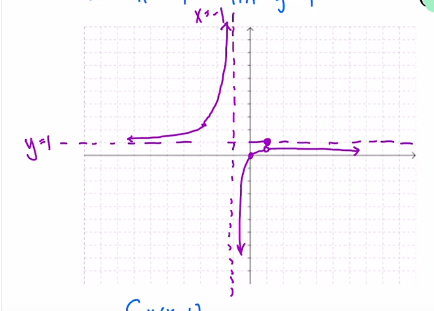
\includegraphics[scale=0.8]{../images/5.png}
        \end{center}

        \pagebreak
        \begin{large}
            \noindent \textbf{Continuity from one side:}
        \end{large}

        \bigbreak \noindent \bigbreak \noindent 
        continuous from the right:
        \begin{align*}
            \lim\limits_{x \to a+}{f \left(x\right) = f \left(a\right)}
        .\end{align*}

        \bigbreak \noindent 
        continuous from the left:
        \begin{align*}
            \lim\limits_{x \to a-}{f \left(x\right) = f \left(a\right)}
        .\end{align*}

        \bigbreak \noindent 
        continuous on an interval: iff f is continuous at every number on the interval 

        \bigbreak \noindent \bigbreak \noindent \bigbreak \noindent 
        \begin{large}
            \textbf{Theorem:}
        \end{large}

        \bigbreak \noindent \bigbreak \noindent 
        \begin{center}
            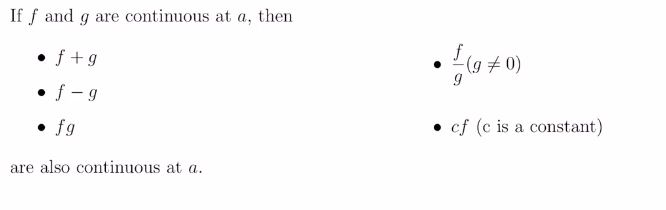
\includegraphics[scale=0.65]{../images/6.png  }
        \end{center}

        \bigbreak \noindent \bigbreak \noindent 
        \begin{center}
            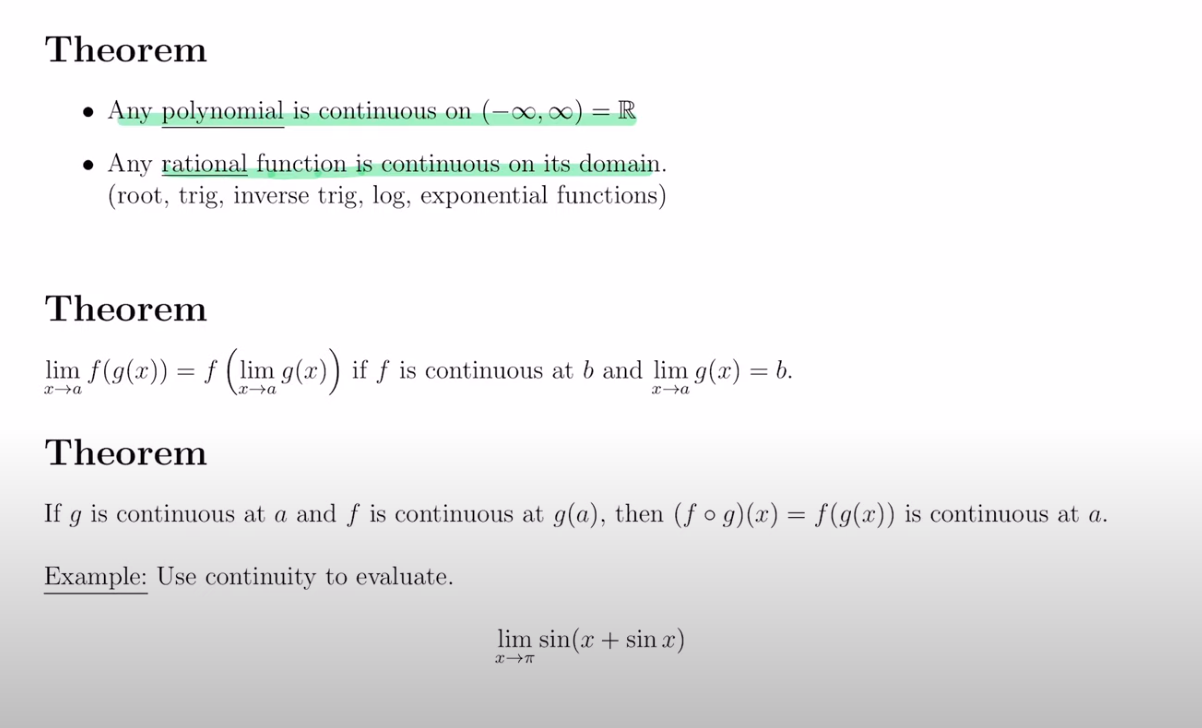
\includegraphics[scale=0.4]{../images/7.png  }
        \end{center}

        \pagebreak
        \begin{large}
            \noindent \textbf{Example: Use Continuity to Evaluate: }
        \end{large}

        \begin{align*}
            \lim\limits_{x \to \pi}{\sin \left(x+\sin x\right)}
        .\end{align*}

        \bigbreak \noindent 
        By the theorem, sin is continuous on its domain, which is $\mathbb{R}$

        \bigbreak \noindent 
        \textbf{So:}
        \begin{align*}
            \sin \left( \lim\limits_{x \to \pi}{ \left(x + \sin x\right)}\right) 
        .\end{align*}

        \bigbreak \noindent 
        So we plug in $\pi$ for x, and since sin $\left(\pi\right)$ = 0, We are just left with:

        \begin{align*}
            \sin \left(\pi+0\right) \\ 
            = 0 
        .\end{align*}

        \bigbreak \noindent 
        Because the sin of $\pi$ is zero.

        \pagebreak
        \begin{Large}
            \noindent \textbf{The Intermediate Value Theorem:}
        \end{Large}

        \bigbreak \noindent \bigbreak \noindent 
        Suppose f is continuous on [a, b]. Let N be any number between f(a) and f(b), where
        f(a) $\neq$ f(b). Then There exists c $\in$ (a,b) such that f(c) = N

        \bigbreak \noindent \bigbreak \noindent 
        \begin{center}
            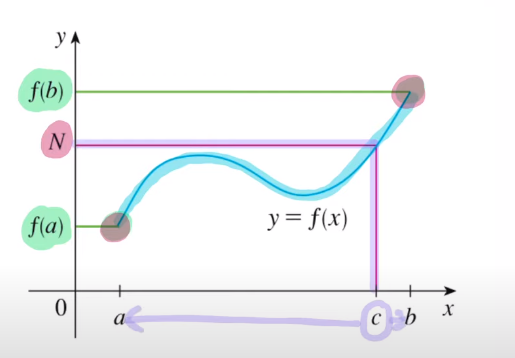
\includegraphics[scale=0.7]{../images/8.png}
        \end{center}

        \bigbreak \noindent \bigbreak \noindent 
        \begin{large}
            \noindent \textbf{Example: Use the IVT to show that there is a root of f(x) = $\sqrt[3]{x} -1 + x$ in (0,1)}
        \end{large}

        \bigbreak \noindent \bigbreak \noindent \bigbreak \noindent 
        \textbf{1.) Show that f is continuous on [0,1]}

        \bigbreak \noindent 
        By theorem, we know that f is continuous on its domain because its a sum of a polynomial
        and a radical function.

        \bigbreak \noindent 
        \textbf{Because the index on the radical is odd, the domain in $\mathbb{R}$}, and [0,1] 
        lies in the domain on $\mathbb{R}$.

        \bigbreak \noindent \bigbreak \noindent 
        \textbf{2.) Show that f(0) $\neq$ f(1)} 

        \bigbreak \noindent 
        so f(0):
        \begin{align*}
            \sqrt[3]{0}-1 + 0 \\ 
            = -1
        .\end{align*}

        \bigbreak \noindent 
        f(1):
        \begin{align*}
            \sqrt[3]{1}-1 + 1 \\ 
            = 1
        .\end{align*}

        \bigbreak \noindent 
        As you can see these 2 function values do not equal eachother

        \bigbreak \noindent \bigbreak \noindent 
        \textbf{3.) Show that n $\in$ (f(0), f(1)}

        \bigbreak \noindent 
        If they are asking for a root, then N = 0, and we can see that 0 $\in$ (-1,1)

        \pagebreak
        \begin{Large}
            \noindent \textbf{One-Sided Continuity:}
        \end{Large}

        \bigbreak \noindent \bigbreak \noindent 
        continuous from the right:
        \begin{align*}
            \lim\limits_{x \to a+}{f \left(x\right) = f \left(a\right)}
        .\end{align*}

        \bigbreak \noindent 
        continuous from the left:
        \begin{align*}
            \lim\limits_{x \to a-}{f \left(x\right) = f \left(a\right)}
        .\end{align*}
    
        \bigbreak \noindent \bigbreak \noindent 
        \nt{If $\lim\limits_{x \to a}{f \left(x\right)}$ \textbf{\textit{Exists,}} Then you dont have
            to worry what side the Continuity is coming from
        } 
        
        \bigbreak \noindent 
        \begin{center}
            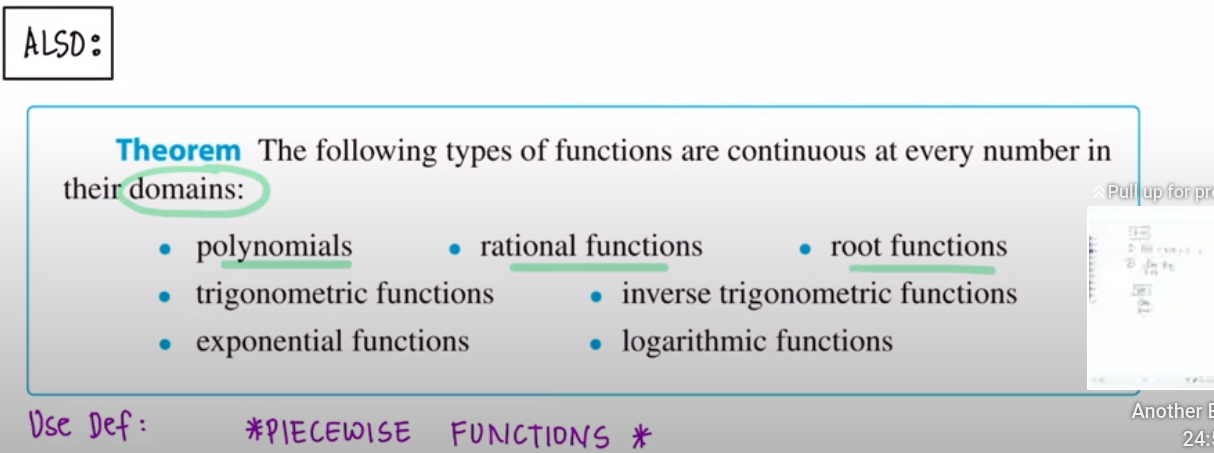
\includegraphics[scale=0.4]{../images/9.png}
        \end{center}

        \nt{You only have to be carefull with root functions if \textbf{n} is \textbf{\textit{even}}}

        \bigbreak \noindent 
        Remember you need to check conditions 1-3 on \textbf{\textit{piecewise functions}}

        \pagebreak
        \begin{large}
            \noindent \textbf{Example 1: Find the numbers at which f is Discontinuous, At which of
                these numbers if f continuous form the right, from the left, or neither, and then
                sketch the graph.
            }
        \end{large}

        \bigbreak \noindent \bigbreak \noindent 
           \begin{equation}
            f \left(x\right)=
                \begin{cases}
                    x^2 & \text{if } x < -1  \\
                     x & \text{if } -1 \leq x < 1 \\
                     \frac{1}{x} & \text{if } x \geq 1 
                \end{cases}
            \end{equation}

        \bigbreak \noindent 
        By theorem, that on ($-\infty$, -1) and (-1,1) f(x) is a polynomial. So it is continuous.

        \bigbreak \noindent 
        by theorem, on (1, $\infty$), f(x) is a rational function, so it will be continuous on its domain.
        So x cannot be 0. \textbf{But (1, $\infty$)} does not include zero, so we are in the clear

        \bigbreak \noindent 
        So we only need to investigate \textbf{\textit{2 values}, at x = -1, and x = 1}, because
        that is where the domain splits in the piecewise function.

        \bigbreak \noindent 
        \textbf{So we will start by investigating x = -1}

        \bigbreak \noindent 
        \textbf{1.)}
        \begin{align*}
            f \left(-1\right) = -1
        .\end{align*}

        \bigbreak \noindent  
        We plug this into the middle portion of our piecewise function because this 
        is where the value \textbf{\textit{-1}} falls.

        \bigbreak \noindent 
        \textbf{2.)}
        \begin{align*}
            \lim\limits_{x \to -1}{f \left(x\right)}
        .\end{align*}

        \bigbreak \noindent 
        We must check the limit from both sides, 

        \bigbreak \noindent 
        \textbf{Left:}
        
        \begin{align*}
            \lim\limits_{x \to -1-}{x^2} = \left(-1\right)^2 \\ 
            = 1
        .\end{align*}

        \bigbreak \noindent 
        We use the first portion of the piecewise function because we are checking for values
        \textbf{\textit{smaller}} than -1

        \bigbreak \noindent 
        \textbf{Right:}

        \begin{align*}
            \lim\limits_{x \to -1+}{x} = -1
        .\end{align*}

        \bigbreak \noindent 
        Using the Second portion of the piecewise function

        \bigbreak \noindent 
        \textbf{We can see that the limit from the left is not equal to the limit
            from the right
        }

        \bigbreak \noindent 
        \textbf{So we know:}

        \begin{align*}
            \lim\limits_{x \to -1}{f \left(x\right) = DNE}
        .\end{align*}

        \bigbreak \noindent 
        \textbf{This tells us that f(x) is Discontinuities at x = -1}

        \bigbreak \noindent 
        Notice that from step 1, we got f(-1) = -1, and this is \textbf{\textit{the same}} 
        as the right hand limit, so that means that f(x) is continuous from the right at x = -1 

        \pagebreak
        \bigbreak \noindent 
        Now we will investigate at x = 1.

        \bigbreak \noindent 
        \textbf{1.)}
        \begin{align*}
            f \left(1\right) = \frac{1}{1} \\ 
            = 1
        .\end{align*}

        \bigbreak \noindent 
        \textbf{2.)} 
        \begin{align*}
            \lim\limits_{x \to 1}{f \left(x\right)}
        .\end{align*}

        \bigbreak \noindent 
        We must check the limit from both sides, 

        \bigbreak \noindent 
        \textbf{Left:}
        \begin{align*}
            \lim\limits_{x \to 1-}{x} = 1 \\ 
        .\end{align*}

        \bigbreak \noindent 
        \textbf{Right:}
        \begin{align*}
            \lim\limits_{x \to 1+}{ \frac{1}{x}} = \frac{1}{1} \\ 
            =  1
        .\end{align*}

        \bigbreak \noindent 
        \textbf{We can see that the limit from the left \textbf{\textit{is}} equal to the limit 
            from the right, 
        }
        \textbf{So we know:}
        \begin{align*}
            \lim\limits_{x \to 1}{f \left(x\right)} = 1
        .\end{align*}

        \bigbreak \noindent 
        \textbf{This tells us that f(x) is \textbf{\textit{continuous}} at \textbf{1}}

        \bigbreak \noindent \bigbreak \noindent 
        \begin{large}
            \textbf{Graph:}
        \end{large}

        \bigbreak \noindent \bigbreak \noindent 
        \begin{center}
            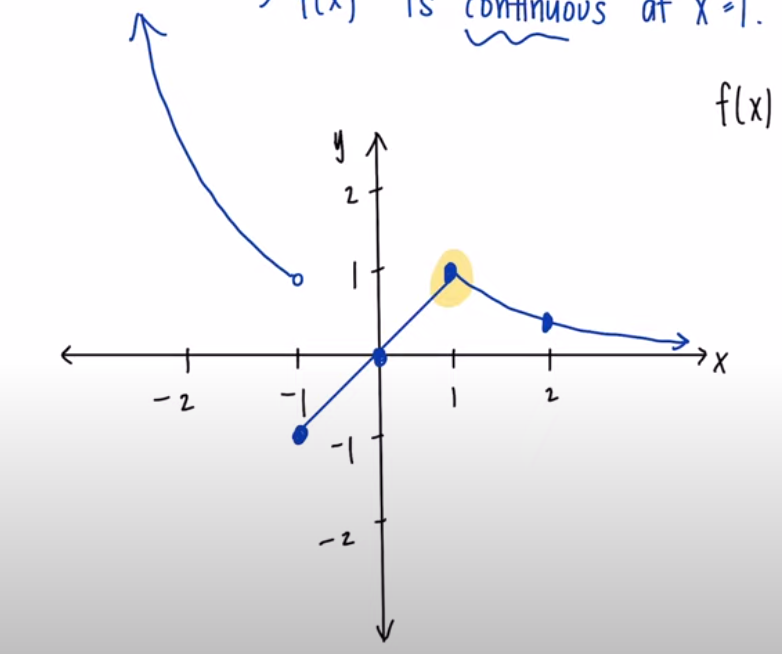
\includegraphics[scale=0.4]{../images/10.png}
        \end{center}


        \pagebreak \bigbreak \noindent
        \begin{Large}
            \textbf{2.6: Limits at infinity, Asymptotes:}
        \end{Large}

        \bigbreak \noindent \bigbreak \noindent \bigbreak \noindent 
        \begin{center}
            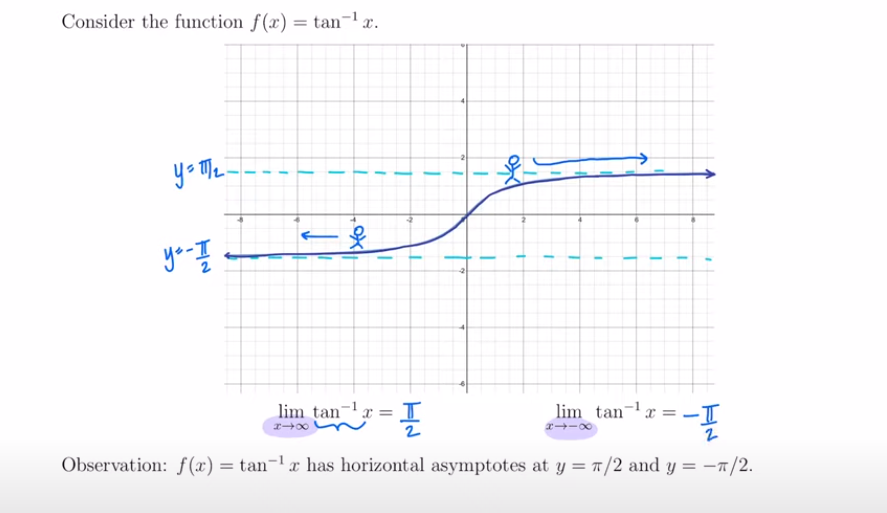
\includegraphics[scale=0.55]{../images/11.png}
        \end{center}

        \bigbreak \noindent \bigbreak \noindent 
        \begin{large}
            \textbf{Definition: The line y = L is a Horizontal Asymptote of y = f(x) if}
        \end{large}

        \begin{align*}
            \lim\limits_{x \to \infty}{f(x)} = L
        .\end{align*}

        \bigbreak \noindent 
        \begin{center}
            or
        \end{center}

        \begin{align*}
            \lim\limits_{x \to - \infty}{f(x) = L}
        .\end{align*}


        \bigbreak \noindent \bigbreak \noindent 
        \begin{large}
            \textbf{Example: for the function g whos graph is given, find the following:}
        \end{large}

        \bigbreak \noindent \bigbreak \noindent 
        \begin{center}
            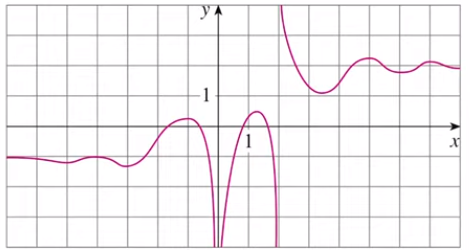
\includegraphics[scale=0.55]{../images/12.png}
        \end{center}

        \pagebreak \bigbreak \noindent
        \textbf{a.) $\lim\limits_{x \to \infty}{g(x)}$ = 2 }

        \bigbreak \noindent 
        \textbf{b.) $\lim\limits_{x \to - \infty}{g(x)}$ = -1}

        \bigbreak \noindent 
        \textbf{c.) $\lim\limits_{x \to 2}{g(x)}$ = ? }

        \bigbreak \noindent 
        We must consider the limit from the \textbf{\textit{left}} and \textbf{\textit{right}} sides.

        \bigbreak \noindent 
        \textbf{So:}

        \begin{align*}
            \lim\limits_{x \to 2+ }{g(x)} = \infty
        .\end{align*}

        \bigbreak \noindent 
        We can see that as we approach 2 from the right, the graph is
        \textbf{\textit{Increasing without bound}}, so the limit is $\infty$

        \bigbreak \noindent 
        \textbf{Now:}

        \begin{align*}
            \lim\limits_{x \to 2-}{g(x)} = - \infty
        .\end{align*}

        \bigbreak \noindent 
        We can see that as we approach 2 from the right, the graph is
        \textbf{\textit{Decreasing without bound}}, so the limit is - $\infty$

        \bigbreak \noindent 
        Since the limit from the left does not equal the limit from the right, 
        the limit as x $\rightarrow$ 2 of g(x) \textbf{\textit{DNE}}

        \bigbreak \noindent \bigbreak \noindent 
        \textbf{d.)} $\lim\limits_{x \to 0}{g(x)} = ? $

        \bigbreak \noindent 
        Here we can see that from the left and right, the limit is approaching - $\infty$

        \bigbreak \noindent 
        \textbf{Therefore,}
        \begin{align*}
           \lim\limits_{x \to 0}{g(x) = - \infty} 
        .\end{align*}

        \bigbreak \noindent \bigbreak \noindent 
        \textbf{e.) $\lim\limits_{x \to -2+}{g(x)}$ = -0.4}

        \bigbreak \noindent 
        This limit of -0.4 is an approximation.

        \bigbreak \noindent  \bigbreak \noindent 
        \textbf{f.) The equations of the Asymptotes are:}

        \begin{align*}
            \text{H.A:}\ y = 2, y = -1 \\
            \text{V.A:}\ x = 0, x = 2
        .\end{align*}

        \pagebreak \bigbreak \noindent
        \begin{large}
            \textbf{Consider: $f(x) = \frac{1}{x}$}
        \end{large}

        \bigbreak \noindent \bigbreak \noindent 
        \begin{center}
            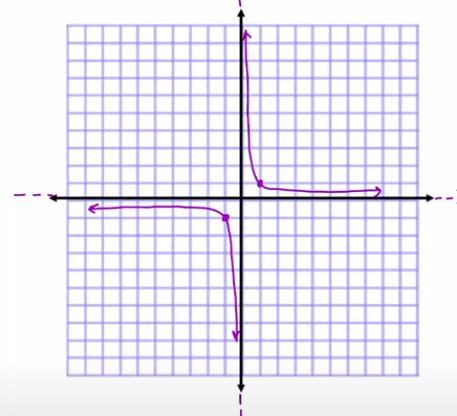
\includegraphics[scale=0.5]{../images/13.png}
        \end{center}

        \bigbreak \noindent 
        \begin{center}
            Our points here for the \textbf{\textit{Reciprical Function}} are (1,1) and (-1,-1)
        \end{center} 

        \bigbreak \noindent \bigbreak \noindent 
        \textbf{Find:}

        \bigbreak \noindent 
        \textbf{a.) $\lim\limits_{x \to \infty}{\frac{1}{x}}$}

        \bigbreak \noindent 
        We can see that as we approach $\infty$ on x the graph is going towards \textbf{\textit{zero}}

        \bigbreak \noindent 
        \textbf{Therefore:}

        \begin{align*}
            \lim\limits_{x \to \infty}{ \frac{1}{x}} = 0
        .\end{align*}

        \bigbreak \noindent \bigbreak \noindent 
        \textbf{b.) $\lim\limits_{x \to - \infty}{ \frac{1}{x}}$}

        \bigbreak \noindent 
        We can see that as we approach - $\infty$ on x the graph is also going towards \textbf{\textit{zero}}

        \bigbreak \noindent 
        \textbf{Therefore:}

        \begin{align*}
            \lim\limits_{x \to - \infty}{ \frac{1}{x} = 0}
        .\end{align*}

        \pagebreak \bigbreak \noindent
        \begin{large}
            \textbf{Theorem:}
        \end{large}

        \bigbreak \noindent 
        % \begin{align*}
        %     \lim\limits_{x \to \infty}{ \frac{1}{x^r}} = 0\ \text{and} \lim\limits_{x \to - \infty}{ \frac{1}{x^r}} = 0\
        %     \text{if r $>$ 0 and is a rational numebr}
        % .\end{align*}
        $\lim\limits_{x \to \infty}{ \frac{1}{x^r}} = 0\ \text{and} \lim\limits_{x \to - \infty}{ \frac{1}{x^r}} = 0\
        \text{if r $>$ 0 and is a rational numebr}$

        \bigbreak \noindent \bigbreak \noindent 
        \begin{large}
            \noindent \textbf{Examples: Find the limit:}
        \end{large}

        \bigbreak \noindent \bigbreak \noindent 
        \textbf{1.) $\lim\limits_{x \to \infty}{ \frac{3x+5}{x - 4}}$}

        \bigbreak \noindent \bigbreak \noindent 
        \textbf{1.) Divide by the highest degree of the denomonator.}
        
        \bigbreak \noindent \bigbreak \noindent 
        So we are going to divide the numerator and the denomonator by \textbf{\textit{x}}

        \bigbreak \noindent 
        \textbf{So:}

        \begin{align*}
            \lim\limits_{x \to \infty}{ \frac{3 + \frac{5}{x}}{1- \frac{4}{x}}}
        .\end{align*}

        \bigbreak \noindent \bigbreak \noindent 
        \textbf{2.) Take the limit of each of the terms in the numerator and denominator}

        \bigbreak \noindent 
        \textbf{So:}

        \begin{align*}
            \frac{ \lim\limits_{x \to \infty}{3} + \lim\limits_{x \to \infty}{ \frac{5}{x}}}{ \lim\limits_{x \to \infty}{1} - \lim\limits_{x \to \infty}{ \frac{4}{x}}}
        .\end{align*}

        \nt{Remember if we take the limit as x approaches $\infty$ of a \textbf{\textit{ constant that doesn't change}}, over x, the limit \textbf{\textit{will be zero!}}}

        \bigbreak \noindent 
        \textbf{So we have:}

        \begin{align*}
            \frac{3+0}{1-0} \\ 
            = 3
        .\end{align*}

        \bigbreak \noindent \bigbreak \noindent \bigbreak \noindent 
        \begin{large}
            \textbf{Example:}
        \end{large}

        \bigbreak \noindent \bigbreak \noindent 
        \textbf{2.) $\lim\limits_{x \to - \infty}{ \frac{t^2 + 2}{t^3+t^2-1}}$}

        \bigbreak \noindent \bigbreak \noindent 
        \textbf{1.) Again, divide by the highest degree in the denominator, which is \textbf{\textit{$t^3$}}}

        \bigbreak \noindent 
        \textbf{So we will have:}

        \begin{align*}
            \lim\limits_{t \to - \infty}{\frac{ \frac{1}{t} + \frac{2}{t^3}}{ 1 + \frac{1}{t} - \frac{1}{t^3}}}
        .\end{align*}

        \bigbreak \noindent 
        Just like the previous example, if we take the limit of each of the terms in both the 
        numerator and the denominator, we get:

        \begin{align*}
            \frac{0 + 0}{1+0-0}
        .\end{align*}

        \bigbreak \noindent 
        Which is just:

        \begin{align*}
            \frac{0}{1} \\
            = 0
        .\end{align*}

        \bigbreak \noindent 
        \nt{If the degree in the denominator is higher than the degree of the denominator, than the equation 
            of the H.A is automatically \textbf{\textit{y=0}}
        }

        \bigbreak \noindent \bigbreak \noindent 
        \begin{large}
            \textbf{Example:}
        \end{large}

        \bigbreak \noindent 
        \textbf{3.) $\lim\limits_{x \to \infty}{ \frac{x+2}{ \sqrt{9x^2+1}}}$}

        \bigbreak \noindent \bigbreak \noindent 
        \textbf{Recall: $\sqrt{x^2} = \abs{x}$}
        
        \bigbreak \noindent 
        Which is the piecewise:

           \begin{equation}
               \abs{x}=
                \begin{cases}
                    x & \text{if } x \geq 0  \\
                    -x & \text{if } x < 0
                \end{cases}
            \end{equation}

        \bigbreak \noindent 
        \textbf{So we divide numerator and denominator by $\abs{x}$, and we have to look at 
            the piecewise function to retrieve the sign of x, since we are going to \textbf{\textit{positive}}
            $\infty$, we will use the top portion of the piecewise. Because this is for \textbf{\textit{positive}} values 
            of x
        }

        \bigbreak \noindent 
        \textbf{So the numerator will be:}
        
        \begin{align*}
            1 + \frac{2}{x}
        .\end{align*}

        \bigbreak \noindent 
        Then for the denominator, we need to divide by $\sqrt{x^2}$

        \bigbreak \noindent 
        \textbf{So:}

        \begin{align*}
            \sqrt{ \frac{9x^2+1}{x^2}}
        .\end{align*}

        \bigbreak \noindent 
        Which gives us:

        \begin{align*}
            \sqrt{9 + \frac{1}{x^2}}
        .\end{align*}

        \bigbreak \noindent 
        So our equation is:

        \begin{align*}
            \lim\limits_{x \to \infty}{ \frac{1+ \frac{2}{x}}{ \sqrt{9+ \frac{1}{x^2}}}}
        .\end{align*}

        \bigbreak \noindent 
        Now if we take the limit of each term in the numerator and denominator, we get:

        \begin{align*}
            \frac{1+0}{ \sqrt{9+0}}
        .\end{align*}

        \bigbreak \noindent 
        Which is simplifed to:

        \begin{align*}
            \frac{1}{3}
        .\end{align*}

        \bigbreak \noindent \bigbreak \noindent \bigbreak \noindent 
        \begin{large}
            \textbf{Example: Negative $\infty$}
        \end{large}

        \bigbreak \noindent \bigbreak \noindent 
        \textbf{4.) $\lim\limits_{x \to - \infty}{ \frac{ \sqrt{9x^6 - x}}{x^3 + 1}}$}

        \bigbreak \noindent 
        Notice that we have $\sqrt{x^6}$, which means we have $\abs{x^3}$

        \bigbreak \noindent 
        \nt{We dont need to do absolute value with piecewise for terms like $\sqrt{x^8}$,
            this is because if it simplifes to x with an \textbf{\textit{even power}}, 
            we know that any value plugged in for x will be even automatically. 
        }

        \bigbreak \noindent 
        So we rewrite $\abs{3}$ as piecewise

        \bigbreak \noindent 
        \textbf{So:}

           \begin{equation}
               \abs{3}=
                \begin{cases}
                    x^3 & \text{if } x \geq 0 \\
                    -x^3 & \text{if } x < 0  
                \end{cases}
            \end{equation}

        \bigbreak \noindent 
        So now we check which way the limit is going to determine which part of the piecewise function
        we will use, since we are going to - $\infty$, we will use the \textbf{\textit{bottom}} portion of the 
        piecewise.

        \bigbreak \noindent 
        So for the numerator we have:

        \begin{align*}
            \sqrt{ \frac{9x^6-x}{x^6}} 
        .\end{align*}

        \bigbreak \noindent 
        Which is:
        
        \begin{align*}
            \sqrt{ \frac{9x^6}{x^6} - \frac{x}{x^6}}
        .\end{align*}

        \bigbreak \noindent 
        Which simplifies to:

        \begin{align*}
            -\sqrt{9 - \frac{1}{x^5}}
        .\end{align*}

        \bigbreak \noindent 
        Notice we put a \textbf{\textit{Negative sign} infront of the equation, this is because we
            used the bottom portion of the piecewise function, this is important
        }

        \bigbreak \noindent 
        \textbf{And for the denominator, we divide by $x^3$, so we will have:}

        \begin{align*}
            \frac{x^3}{x^3} + \frac{1}{x^3}
        .\end{align*}

        \bigbreak \noindent 
        Which simplifes to:
        
        \begin{align*}
            1 + \frac{1}{x^3}
        .\end{align*}

        \bigbreak \noindent 
        So our full equation would be:

        \begin{align*}
            \lim\limits_{x \to - \infty}{ \frac{- \sqrt{9- \frac{1}{x^5}}}{1 + \frac{1}{x^3}}}
        .\end{align*}

        \bigbreak \noindent 
        And now if we take the limits for each of the terms, we get:

        \begin{align*}
            \frac{- \sqrt{9 - 0}}{1 + 0}
        .\end{align*}

        \bigbreak \noindent 
        Which simplifes to:

        \begin{align*}
            -3
        .\end{align*}

        \bigbreak \noindent \bigbreak \noindent 
        \begin{large}
            \textbf{Last Example:}
        \end{large}

        \bigbreak \noindent 
        \textbf{5.) $\lim\limits_{x \to \infty}{ \frac{x^3-2x+3}{5-2x^2}}$}

        \bigbreak \noindent \bigbreak \noindent  
        So we divide by the highest degree in the denominator: \textbf{\textit{$x^2$}}

        \bigbreak \noindent 
        \textbf{So:}
        \begin{align*}
            \lim\limits_{x \to \infty}{ \frac{x - \frac{2}{x} + \frac{3}{x}}{ \frac{5}{x} - 2}}
        .\end{align*}

        \bigbreak \noindent 
        Now we take the limit of each of the terms:

        \begin{align*}
            \frac{ \infty - 0 + 0}{0 - 2}            
        .\end{align*}

        \bigbreak \noindent 
        Which simplifies to:
        \begin{align*}
            \frac{ \infty}{-2} \\ 
            = - \infty
        .\end{align*}

        \pagebreak \bigbreak \noindent
        \begin{large}
            \textbf{Infinite Limits at Infinity:}
        \end{large}

        \bigbreak \noindent  \bigbreak \noindent  \bigbreak \noindent 
        \textbf{Consider f(x) = $x^3$}

        \bigbreak \noindent \bigbreak \noindent 
        \begin{center}
            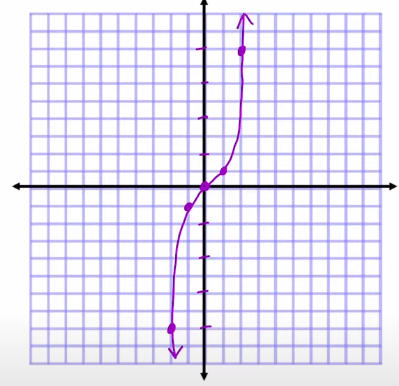
\includegraphics[scale=0.5]{../images/15.png}
        \end{center}

        \bigbreak \noindent 
        \textbf{1.) $\lim\limits_{x \to \infty}{x^3} = \infty $}

        \bigbreak \noindent 
        \textbf{2.) $\lim\limits_{x \to - \infty}{x^3} = - \infty$}

        \bigbreak \noindent 
        \textbf{The term we use to describe this situation is \textbf{\textit{end behavior}}}

        \bigbreak \noindent \bigbreak \noindent \bigbreak \noindent 
        \begin{large}
            \textbf{Recap:}
        \end{large}

        \bigbreak \noindent 
        \begin{large}
            \textbf{H.A:}
        \end{large}

        \bigbreak \noindent 
        \textbf{Take $\lim\limits_{x \to \infty}{f(x)}$ \textbf{\textit{and}} $\lim\limits_{x \to - \infty}{f(x)}$}

        \bigbreak \noindent 
        If f(x) = some constant \textbf{\textit{c}}, then H.A is y = c 

        \bigbreak \noindent \bigbreak \noindent 
        \begin{large}
            \textbf{V.A:}
        \end{large}

        \bigbreak \noindent 
        x = k, where \textbf{\textit{x - k} is a factor of the \textbf{\textit{denominator only!}}}

        \bigbreak \noindent \bigbreak \noindent  \bigbreak \noindent 
        \begin{large}
            \textbf{Example: Find the Horizontal Asymptotes and Vertical Asymptotes:}
        \end{large}

        \begin{align*}
            y = \frac{1 + x^4}{x^2 - x^4}
        .\end{align*}

        \bigbreak \noindent 
        So for \textbf{\textit{H.A}, we want to take the limit of both \textbf{\textit{positve and negaitive infinity.}}}

        \bigbreak \noindent 
        \textbf{So:}

        \begin{align*}
            \lim\limits_{x \to \infty}{ \frac{1 + x^4}{x^2 - x^4}}
        .\end{align*}

        \bigbreak \noindent 
        So divide both sides by the highest degree in the denominator, \textbf{\textit{$x^4$}}
        
        \begin{align*}
            \lim\limits_{x \to \infty}{ \frac{\frac{1}{x^4} + 1}{ \frac{1}{x^2} - 1}} 
        .\end{align*}

        \bigbreak \noindent 
        Now take the limits of each term and get:

        \begin{align*}
           \frac{0 + 1}{0 - 1} \\
        = \frac{1}{-1} \\ 
        = -1
        .\end{align*}

        \bigbreak \noindent 
        Same result for $\lim\limits_{x \to - \infty}{}$, \textbf{So H.A is y = -1}

        \bigbreak \noindent \bigbreak \noindent 
        \textbf{Now for V.A:}

        \bigbreak \noindent 
        Start by factoring the equation:

        \begin{align*}
            y = \frac{1 + x^4}{x^2 \left(1 - x^2\right)}
        .\end{align*}

        \bigbreak \noindent 
        Denominator factors further by using \textbf{\textit{Difference of squares:}}

        \begin{align*}
            y = \frac{1 + x^4}{x^2 \left(1 + x\right) \left(1 - x\right)}
        .\end{align*}

        \bigbreak \noindent 
        Since we cant cancel out any common factors, this equation is fully factored and simplified,
        and the zeros of the Denominator is going to be the equations for our vertical Asymptotes.

        \bigbreak \noindent 
        \textbf{So:}

        \begin{align*}
            x = 0, x = -1, x = 1
        .\end{align*}

        \pagebreak \bigbreak \noindent
        \begin{Large}
            \textbf{2.7: Derivatives and rates of change:}
        \end{Large}

        \bigbreak \noindent \bigbreak \noindent 
        \begin{large}
            \textbf{Back to tangent lines:}
        \end{large}

        \bigbreak \noindent \bigbreak \noindent 
        \begin{center}
            \textbf{Recall:}
        \end{center}
        \begin{align*}
            m_{pq} = \frac{f(x) - f(a)}{x - a}\ \text{is the slope of the \textbf{\textit{Secent line}}} 
        .\end{align*}

        \bigbreak \noindent 
        \begin{center}
            \textbf{And:}
        \end{center}
        \begin{align*}
            \lim\limits_{q \to p}{m_{pq} = m}\ \text{is the slope of the tangent line at point P}
        .\end{align*}

        \bigbreak \noindent 
        \begin{center}
            \textbf{Another way to state that is the following:}
        \end{center}
        \begin{align*}
            \lim\limits_{x \to a}{ \frac{f(x) - f(a)}{x-a} = m }
        .\end{align*}

        \bigbreak \noindent 
        \begin{center}
            \textbf{Another way to expess the above slope formula is base on the following:}
        \end{center}

        \bigbreak \noindent 
        \begin{align*}
            Q \left(a+h, f \left(a+h\right)\right)
        .\end{align*}

        \bigbreak \noindent 
        \begin{center}
            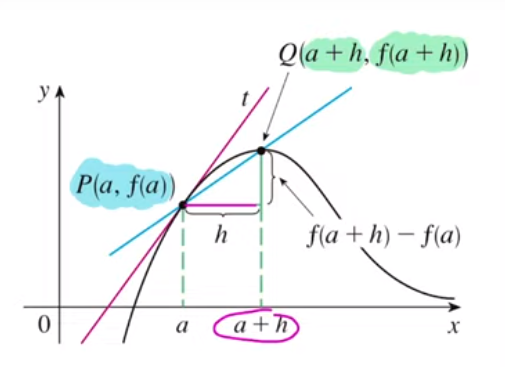
\includegraphics[scale=0.5]{../images/20.png}
        \end{center}

        \bigbreak \noindent 
        The slope of the \textbf{\textit{Secent Line}} would be:

        \begin{align*}
            m_{pq} = \frac{f \left(a+h\right) - f \left(a\right)}{a + h - a} \\
            = \frac{f \left(a+h\right) - f(a)}{h}
        .\end{align*}

        \bigbreak \noindent 
        Slope of the tangent line would be:

        \begin{align*}
           \lim\limits_{h \to 0}{ \frac{f \left(a + h\right) - f(a)}{h}} 
        .\end{align*}

        \bigbreak \noindent 
        This is the \textbf{\textit{Difference quotient}}

        \pagebreak \bigbreak \noindent
        \begin{large}
            \textbf{Example: Find an equation of the tangent line to the curve $y = 2x^3 - 5x$ at the point (-1,3)}
        \end{large}

        \bigbreak \noindent 
        \begin{center}
            Note that P(-1,3) is (a, f(a))
        \end{center}

        \bigbreak \noindent 
        So we need:
        \begin{enumerate}
            \item Point
            \item Slope
        \end{enumerate}

        \bigbreak \noindent 
        We have a point, but we dont have slope since we only have \textbf{\textit{one point}}, So to find the slope
        of the tangent line, we will use the definiton from the previous page. 

        \bigbreak \noindent 
        \begin{center}
            We know:
        \end{center}
        \begin{align*}
            a = 1
        .\end{align*}

        \begin{align*}
            m_{tan} = \lim\limits_{x \to -1}{ \frac{f(x) - f(-1)}{x- \left(-1\right)}} \\ 
            = \lim\limits_{x \to -1}{ \frac{2x^3-5x-3}{x+1}}
        .\end{align*}

        \bigbreak \noindent 
        We cant use direct Substitution, so we need to factor. But we can use \textbf{\textit{synthetic division to factor}}

        \begin{center}
            Synthetic Division:
        \end{center}

        \begin{center}
            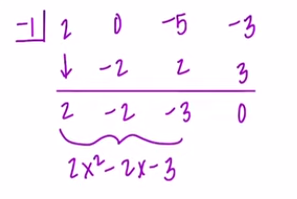
\includegraphics[scale=0.5]{../images/21.png}
        \end{center}

        \bigbreak \noindent 
        \textbf{Explanation:}
        \bigbreak \noindent 
        2 for $x^3$, 0 for $x^2$, -5 for x, and -3, then drop down the 2, multiply by the negative one and
        add down. Then these are the terms.

        \bigbreak \noindent 
        \begin{center}
            So now:
        \end{center}
        \begin{align*}
            \lim\limits_{x \to -1}{ \frac{ \left(2x^2-2x-3\right) \left(x+1\right)}{x+1}} \\ 
            = \lim\limits_{x \to -1}{ \left(2x^2-2x-3\right)}
        .\end{align*}
        \nt{Notice that we added a (x+1) in the numerator of our factored equation after synthetic division.}

        \bigbreak \noindent 
        Now we can plug in -1 into our factored equation and output the limit.

        \begin{align*}
            \lim\limits_{x \to -1}{2 \left(-1\right)^2 + 2 \left(1\right) - 3} \\ 
            = 1
        .\end{align*}
        \bigbreak \noindent 
        Now we can put it all together and find the equation of the tangent line using point slope form:

        \begin{align*}
            y-3 = 1 \left(x- \left(-1\right)\right) \\ 
            y - 3 = x + 1 \\ 
            y = x + 4
        .\end{align*}

        \bigbreak \noindent \bigbreak \noindent 
        \begin{large}
            \textbf{Alteratively, another way to get m:}
        \end{large}

        \begin{align*}
            \lim\limits_{h \to 0}{ \frac{f \left(-1+h\right) - f\left(-1\right)}{h}} \\ 
            = \lim\limits_{h \to 0}{ \frac{2 \left(-1+h\right)^3 - 5 \left(-1+h\right) - 3}{h}}
        .\end{align*}

        \bigbreak \noindent 
        First, foil out $(-1+h)^3$:
        \begin{align*}
            2 \left(h^3 - 3h^2 + 3h -1\right) \\ 
            = 2h^3 - 6h^2 + 6h -2
        .\end{align*}

        \bigbreak \noindent 
        Then, distribute $-5$ to $(-1+h)$

        \begin{align*}
            = -5h + 5
        .\end{align*}

        \bigbreak \noindent 
        So all together we have:

        \begin{align*}
            \frac{2h^3-6h^2+6h-2-5h+5-3}{h} \\ 
            = \frac{2h^3 -6h^2 + h}{h}
        .\end{align*}

        \bigbreak \noindent 
        Now, factor out an h:

        \begin{align*}
            \frac{h \left(2h^2-6h+1\right)}{h}  
        .\end{align*}

        \bigbreak \noindent 
        Cancel out the common factor:

        \begin{align*}
            2h^2-6h+1
        .\end{align*}
        \bigbreak \noindent 
        Now plug in zero for h 

        \begin{align*}
            2 \left(0\right)^2 - 6 \left(0\right) + 1 \\ 
            = 1
        .\end{align*}
        \bigbreak \noindent 
        So you see we got the same answer of \textbf{\textit{1}}:

        \pagebreak \bigbreak \noindent
        \begin{large}
            \textbf{Velocites:}
        \end{large}

        \bigbreak \noindent \bigbreak \noindent 
        \textbf{Suppose an object moves along a straight line according to an equation of motion s = f(t)}
        \begin{align*}
            v_{ave} = \frac{Displacement}{Time} = \frac{f(a+ h) - f(a)}{h}
        .\end{align*}

        \bigbreak \noindent 
        \textbf{For time interval $t = a$ to $t = a + h$}
        \begin{center}
            \textbf{And:}
        \end{center}
        \begin{align*}
            v_{inst} = \lim\limits_{h \to 0}{ \frac{f(a+h) - f(a)}{h}}
        .\end{align*}

        \bigbreak \noindent 
        \textbf{At time $t = a$}
        \begin{center}
            \textbf{Or:}
        \end{center}
        \begin{align*}
            \lim\limits_{t \to a}{ \frac{f(t) - f(a)}{t -a}}
        .\end{align*}

        \bigbreak \noindent 
        \nt{Speed = $\abs{Velocity}$}

        \bigbreak \noindent \bigbreak \noindent 
        \begin{large}
            \textbf{Example: If a ball is thrown upward, it height after $t$ seconds 
            is $y= 40t-16t^2$. find the velocity when t= 3
        }
        \end{large}
        \bigbreak \noindent \bigbreak \noindent \bigbreak \noindent 
        \begin{align*}
            v_{inst} = \lim\limits_{h \to 0}{ \frac{f(3+h) - f(3)}{h}} \\ 
            = \lim\limits_{h \to 0}{ \frac{[40(3+h) - 16(3+h)^2] - [40 \cdot 3 - 16 \cdot 3^2]}{h}}
        .\end{align*}
        \bigbreak \noindent 
        Now distribute out everything:
        \begin{align*}
            \lim\limits_{h \to 0}{ \frac{120+40h-144-96h-16h^2+24}{h}}
        .\end{align*}
        \bigbreak \noindent 
        Combine Like terms:
        \begin{align*}
            \lim\limits_{h \to 0}{ \frac{-56h-16h^2}{h}}
        .\end{align*}
        \bigbreak \noindent 
        Factor out an \textbf{\textit{h}}
        \begin{align*}
            \lim\limits_{h \to 0}{ \frac{h \left(-56-16h\right)}{h}} \\
            = \lim\limits_{h \to 0}{-56-16h}
        .\end{align*}
        \bigbreak \noindent 
        Now plug in zero
        \begin{align*}
            -56 -16 \left(0\right) \\ 
            = -56 m \diagdown s
        .\end{align*}

        \pagebreak \bigbreak \noindent
        \begin{large}
            \textbf{Derivatives:}
        \end{large}
        \bigbreak \noindent \bigbreak \noindent \bigbreak \noindent   
        \textbf{Above Formulas are given a special name:}
        \bigbreak \noindent 
        \textbf{The Derivative of a function f at a number a is:}
        \begin{align*}
            f\prime (a) = \lim\limits_{h \to 0}{ \frac{f(a+h) - f(a)}{h}}
        .\end{align*}
        \bigbreak \noindent 
        \begin{center}
            \textbf{Or:}
        \end{center}
        \begin{align*}
            f\prime (a) = \lim\limits_{x \to a}{ \frac{f(x) - f(a)}{x -a }}
        .\end{align*}

        \bigbreak \noindent 
        \textbf{On a graph $f\prime (a) = m_{tan}$ and represents Instantaneous rate of change}

        \bigbreak \noindent \bigbreak \noindent 
        \begin{large}
            \textbf{Example: Find $f\prime (a)$ if f(x) = $\frac{x^2+1}{x-2}$}
        \end{large}
        
        \bigbreak \noindent \bigbreak \noindent 
        \begin{align*}
            \lim\limits_{h \to 0}{ \frac{ \frac{ \left(a+h\right)^2 + 1}{ \left(a+h\right)-2} - \frac{a^2+1}{a-2}}{h}}
        .\end{align*}

        \bigbreak \noindent 
        So we multiply by the lcd of the \textbf{\textit{entire fraction}}, which is $ \frac{ \left(a+h-2\right) \left(a-2\right)}{ \left(a+h-2\right) \left(a-2\right)}$

        \begin{align*}
            \lim\limits_{h \to 0}{ \frac{ \left( \left(a+h\right)^2+1\right) \left(a-2\right) - \left(a^2+1\right) \left(a+h-2\right)}{h \left(a+h-2\right) \left(a-2\right)}} \\ 
            = \lim\limits_{h \to 0}{ \frac{ \left(a^2+2ah+h^2+1\right) \left(a-2\right) - \left(a^3+a^2h-2a^2+a+h-2\right)}{h \left(h+a-2\right)(a-2)}} \\ 
            = \lim\limits_{h \to 0}{ \frac{a^3+2a^2h+ah^2+a-2a^2-4ah-2h^2-2-a^3-a^2h+2a^2-a-h+2}{h \left(a+h-2\right)(a-2)}}
        .\end{align*}
        \bigbreak \noindent 
        Now cancel out terms and combine like terms
        \begin{align*}
            \lim\limits_{h \to 0}{ \frac{a^2h+ah^2-4ah-2h^2-h}{h (a+h-2)(a-2)}} \\ 
            = \lim\limits_{h \to 0}{ \frac{h (a^2+ah-4a-2h-1)}{h (a+h-2)(a-2)}} \\
            = \lim\limits_{h \to 0}{ \frac{a^2+ah-4a-2h-1}{(a+h-2)(a-2)}}
        .\end{align*}
        \bigbreak \noindent 
        Now plug in zero for h
        \begin{align*}
            \frac{a^2+a \cdot 0 - 4a -2 \cdot 0 -1}{(a+0-2)(a-2)} \\
            = \frac{a^2-4a-1}{(a-2)^2}
        .\end{align*}

        \pagebreak \bigbreak \noindent
        \begin{large}
            \textbf{Example: If f(t) = $t^{-1} -t$, find the velocity and speed when $t=5$}
        \end{large}

        \bigbreak \noindent \bigbreak \noindent 
        So we can use either formula listed above, \textbf{\textit{Either:}}
        \begin{align*}
            \lim\limits_{h \to 0}{ \frac{f(5+h) - f(5)}{h}} 
        .\end{align*}

        \bigbreak \noindent 
        \begin{center}
            \textbf{or}
        \end{center}

        \begin{align*}
            \lim\limits_{t \to 5}{ \frac{f(t) - f(5)}{t-5}}
        .\end{align*}

        \bigbreak \noindent 
        We are going to use the bottom one:
        \bigbreak \noindent 
        \nt{$t^{-1}$ is the same as $\frac{1}{t}$}

        \bigbreak \noindent 
        \begin{align*}
            \lim\limits_{t \to 5}{ \frac{ \frac{1}{t} - t  - ( \frac{1}{5} - 5)}{t -5}}
        .\end{align*}

        \bigbreak \noindent 
        So we want to multiply by the lcd of the entire expression to \textbf{\textit{clear out the fractions}},
        in this case the \textbf{\textit{lcd}} is \textbf{5t}

        \begin{align*}
            \lim\limits_{t \to 5}{ \frac{5 - 5t^2 - t-25t}{(t-5)(5t)}} \\ 
            = \lim\limits_{t \to 5}{ \frac{-5t^2+24t+5}{5t(t-5)}}
        .\end{align*}

        \bigbreak \noindent 
        To make things easier for the numerator, we want to factor out the negative in the \textbf{\textit{leading term}}

        \begin{align*}
            \lim\limits_{t \to 5}{ \frac{- (5t^2-24t-5)}{5t(t-5)}}
        .\end{align*}

        \bigbreak \noindent 
        Now factor the numerator:
        \begin{align*}
            \lim\limits_{t \to 5}{ \frac{- (5t+1)(t-5)}{5t(t-5)}} \\
            = \lim\limits_{t \to 5}{ \frac{-(5t+1)}{5t}}
        .\end{align*}

        \bigbreak \noindent 
        Now use direct Substitution

        \begin{align*}
            \frac{- (5 \cdot 5 + 1)}{5 \cdot 5} \\ 
            = - \frac{26}{25}
        .\end{align*}
        \bigbreak \noindent 
        So \textbf{Velocity: $ \frac{-26}{25}$ $u \diagdown s$} 
        \bigbreak \noindent 
        And \textbf{speed: $\abs{ \frac{-26}{25}} = \frac{26}{25}$ $u \diagdown s$ }

\end{document}

